\begin{figure}[t]
\vspace*{-2ex}
\centering
\begin{subfigure}{.18\textwidth}

\includegraphics[width=\linewidth]{tasks/dmc}
\caption{Control Suite}
\end{subfigure}\hfill
\begin{subfigure}{.18\textwidth}

\includegraphics[width=\linewidth]{tasks/atari}
\caption{Atari}
\end{subfigure}\hfill
\begin{subfigure}{.18\textwidth}
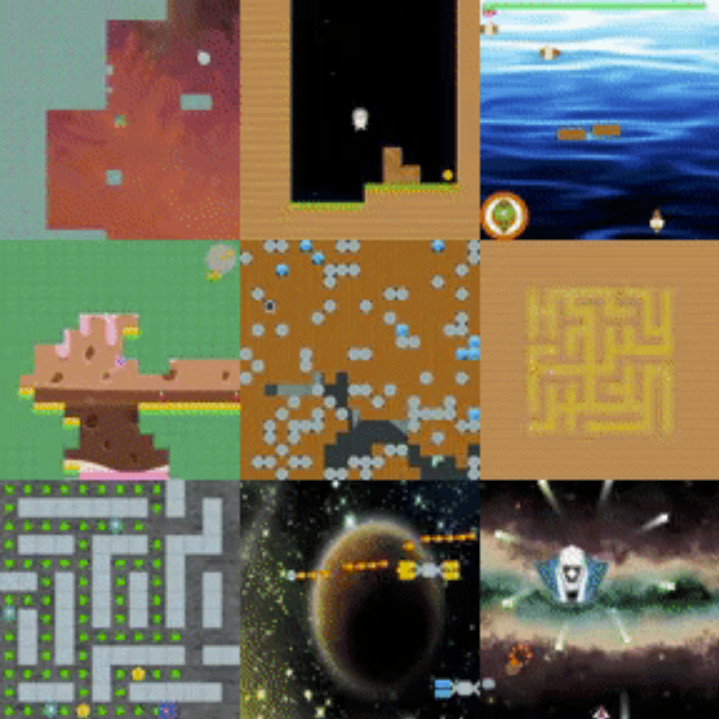
\includegraphics[width=\linewidth]{tasks/procgen}
\caption{ProcGen}
\end{subfigure}\hfill
\begin{subfigure}{.18\textwidth}

\includegraphics[width=\linewidth]{tasks/dmlab}
\caption{DMLab}
\end{subfigure}\hfill
\begin{subfigure}{.18\textwidth}

\includegraphics[width=\linewidth]{tasks/minecraft}
\caption{Minecraft}
\end{subfigure}
\caption{Diverse visual domains used in the experiments. Dreamer succeeds across these domains, ranging from robot locomotion and manipulation tasks over Atari games, procedurally generated ProcGen levels, and DMLab tasks, that require spatial and temporal reasoning, to the complex and infinite world of Minecraft. We also evaluate Dreamer on non-visual domains.}
\label{fig:tasks}
\end{figure}
